\documentclass[12pt]{article}
\usepackage[utf8]{inputenc}
\usepackage[margin=1in]{geometry}
\usepackage{amsmath}\usepackage{amssymb}\usepackage{multicol}\usepackage{enumitem}
\usepackage{pgfplots}\pgfplotsset{compat=1.17}
\setlength{\parindent}{0pt}
\begin{document}

\fbox{\parbox{0.97\linewidth}{\small\textbf{Final answers} (record here --- graded on the answer; show your work):\\[6pt]1.~\underline{\hspace{1.5cm}}\quad 2.~\underline{\hspace{1.5cm}}\quad 3.~\underline{\hspace{1.5cm}}\quad 4.~\underline{\hspace{1.5cm}}\quad 5.~\underline{\hspace{1.5cm}}\quad 6.~\underline{\hspace{1.5cm}}\quad 7.~\underline{\hspace{1.5cm}}\quad 8.~\underline{\hspace{1.5cm}}\quad 9.~\underline{\hspace{1.5cm}}\quad 10.~\underline{\hspace{1.5cm}}\quad 11.~\underline{\hspace{1.5cm}}\quad 12.~\underline{\hspace{1.5cm}}\quad 13.~\underline{\hspace{1.5cm}}}}
\vspace{0.35cm}

\begin{center}{\Large \textbf{Warm-Up: The Discriminant}}\end{center}\vspace{0.2cm}
% Warm-Up: The Discriminant
\textbf{Example (Warm-Up: The Discriminant):}

For $x^2-2x-8=0$, the discriminant is $b^2-4ac=(-2)^2-4(1)(-8)=4+32=36$. Since $36>0$, there are two real solutions.

\vspace{0.2cm}\hrule\vspace{0.35cm}
\textbf{Directions: Compute the discriminant $b^2-4ac$ for each equation and state the number of real solutions.}

\begin{multicols}{2}
\begin{enumerate}[label=\textbf{\arabic*.}, start=1, itemsep=1.3cm]
  \item $\displaystyle x^2+4x+3=0$
  \item $\displaystyle x^2-8x+16=0$
  \item $\displaystyle x^2+2x+5=0$
  \item $\displaystyle 2x^2+3x-2=0$
\end{enumerate}
\end{multicols}
\vspace{0.25cm}\hrule\vspace{0.35cm}

\begin{center}{\Large \textbf{Solve with the Formula}}\end{center}\vspace{0.2cm}
% Solve with the Formula
\textbf{Example (Solve with the Formula):}

Solve $x^2-3x-10=0$. Here $a=1,b=-3,c=-10$, so $x=\dfrac{3\pm\sqrt{9+40}}{2}=\dfrac{3\pm 7}{2}$, giving $x=5$ or $x=-2$.

\vspace{0.2cm}\hrule\vspace{0.35cm}
\textbf{Directions: Solve each equation using the quadratic formula. Show the discriminant, then simplify completely (leave irrational answers in simplest radical form).}

\begin{multicols}{2}
\begin{enumerate}[label=\textbf{\arabic*.}, start=5, itemsep=3cm]
  \item $\displaystyle x^2+8x+15=0$
  \item $\displaystyle x^2-9x+20=0$
  \item $\displaystyle 2x^2+7x-4=0$
  \item $\displaystyle x^2-6x+4=0$
  \item $\displaystyle 3x^2-2x-1=0$
\end{enumerate}
\end{multicols}
\vspace{0.25cm}\hrule\vspace{0.35cm}

\begin{center}{\Large \textbf{Graphical Connection}}\end{center}\vspace{0.2cm}
% Graphical Connection
\textbf{Example (Graphical Connection):}

The parabola $y=x^2-2x-3$ crosses the $x$-axis at its roots. Solving $x^2-2x-3=0$ gives $x=3$ and $x=-1$, matching the $x$-intercepts on the graph.

\begin{center}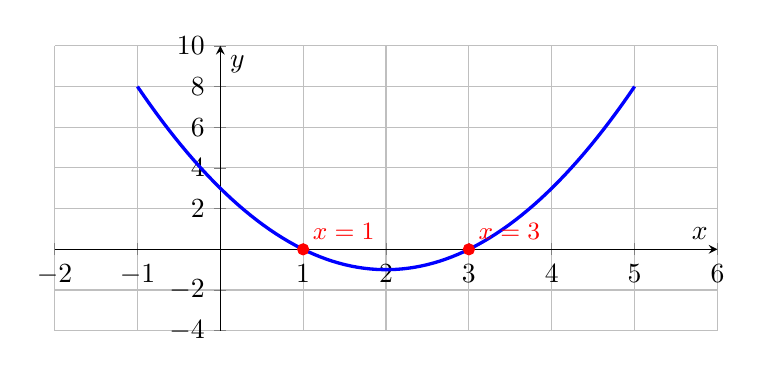
\begin{tikzpicture}
\begin{axis}[axis lines=middle,xlabel=$x$,ylabel=$y$,xmin=-2,xmax=6,ymin=-4,ymax=10,width=10cm,height=5.2cm,grid=both,xtick={-2,-1,1,2,3,4,5,6},ytick={-4,-2,2,4,6,8,10},samples=80]
\addplot[very thick,blue,domain=-1:5]{x^2-4*x+3};
\addplot[only marks,mark=*,red] coordinates {(1,0)};
\node[above right,red,font=\small] at (axis cs:1,0) {$x=1$};
\addplot[only marks,mark=*,red] coordinates {(3,0)};
\node[above right,red,font=\small] at (axis cs:3,0) {$x=3$};
\end{axis}\end{tikzpicture}\end{center}
{\small\centering $y=x^2-4x+3$ with roots at $x=1$ and $x=3$.\par}
\vspace{0.2cm}\hrule\vspace{0.35cm}
\textbf{Directions: Use the graph of $y=x^2-4x+3$ to identify the roots, then verify each one using the quadratic formula.}

\begin{multicols}{2}
\begin{enumerate}[label=\textbf{\arabic*.}, start=10, itemsep=2cm]
  \item Confirm the roots of $x^2-4x+3=0$ using the quadratic formula.
  \item Compute the discriminant of $x^2-4x+3=0$ and explain what its sign tells you about the graph.
\end{enumerate}
\end{multicols}

\vspace{0.2cm}\hrule\vspace{0.3cm}
\textbf{Challenge} (same sheet):\\[4pt]
\begin{multicols}{2}
\begin{enumerate}[label=\textbf{\arabic*.}, start=12, itemsep=2.2cm]
  \item Solve $3x^2-8x+4=0$ using the quadratic formula.
  \item A ball's height in feet is modeled by $h=-16t^2+64t$. Find the times $t$ (in seconds) when the ball is at height $h=0$.
\end{enumerate}
\end{multicols}

\newpage

\begin{center}{\Large \textbf{Answer Key --- fully worked}}\end{center}
\vspace{0.25cm}
\textbf{Procedure:} Write the equation in standard form $ax^2+bx+c=0$.; Identify the values of $a$, $b$, and $c$.; Compute the discriminant $b^2-4ac$ to predict the number of real solutions.; Substitute $a$, $b$, and $c$ into $x=\dfrac{-b\pm\sqrt{b^2-4ac}}{2a}$.; Simplify the square root and reduce the fraction to find both solutions.; Check each solution by substituting it back into the original equation..\\[8pt]
\begin{enumerate}[label=\textbf{\arabic*.},itemsep=7pt]
  \item $b^2-4ac=4^2-4(1)(3)=16-12=4>0$ -> two real solutions.
  \item $b^2-4ac=(-8)^2-4(1)(16)=64-64=0$ -> one real (repeated) solution.
  \item $b^2-4ac=2^2-4(1)(5)=4-20=-16<0$ -> no real solutions.
  \item $b^2-4ac=3^2-4(2)(-2)=9+16=25>0$ -> two real solutions.
  \item $a=1,b=8,c=15$; disc $=64-60=4$; $x=\dfrac{-8\pm 2}{2}$ -> $x=-3$ or $x=-5$.
  \item $a=1,b=-9,c=20$; disc $=81-80=1$; $x=\dfrac{9\pm 1}{2}$ -> $x=5$ or $x=4$.
  \item $a=2,b=7,c=-4$; disc $=49+32=81$; $x=\dfrac{-7\pm 9}{4}$ -> $x=\dfrac{1}{2}$ or $x=-4$.
  \item $a=1,b=-6,c=4$; disc $=36-16=20$; $x=\dfrac{6\pm\sqrt{20}}{2}=\dfrac{6\pm 2\sqrt{5}}{2}=3\pm\sqrt{5}$.
  \item $a=3,b=-2,c=-1$; disc $=4+12=16$; $x=\dfrac{2\pm 4}{6}$ -> $x=1$ or $x=-\dfrac{1}{3}$.
  \item $a=1,b=-4,c=3$; disc $=16-12=4$; $x=\dfrac{4\pm 2}{2}$ -> $x=3$ or $x=1$, matching the $x$-intercepts shown on the graph.
  \item disc $=(-4)^2-4(1)(3)=4>0$, which is positive, so the parabola crosses the $x$-axis at two distinct points (two real roots).
  \item $a=3,b=-8,c=4$; disc $=64-48=16$; $x=\dfrac{8\pm 4}{6}$ -> $x=2$ or $x=\dfrac{2}{3}$.
  \item Set $-16t^2+64t=0$: $a=-16,b=64,c=0$; disc $=64^2-4(-16)(0)=4096$; $t=\dfrac{-64\pm 64}{-32}$ -> $t=0$ or $t=4$; since $t=0$ is the launch, the ball returns to $h=0$ at $t=4$ seconds.
\end{enumerate}

\end{document}